\chapter{Proposed research plan}
As discussed in \cref{sec:challenges}, the study of additive manufacturing is a rather challenging task, mainly because industrial interests aimed at improving AM technology are strongly related to issues that span a wide length scale, from meso--scale to the atomistic level. Many phenomena that play a central role in the entire manufacturing process require the synergic collaboration of different approaches to obtain meaningful results.

We can summarize the previous statement in the following way: applications at the industrial level frequently encounter a series of metallurgical problems that must firstly be fully understood to improve quality features of AM produced parts; on the other hand, AM processes are too much complicated to be directly studied by means of atomistic simulations and for this reason several phase field models have been developed to give useful guidelines to industrial applications. However, in many cases even phase field models lack important knowledge of the fundamental phenomena occurring in an AM process, for example during phase transitions. It is in the latter context that atomistic simulations can give a valuable contribution. 

During the first year of the PhD program, a considerable amount of time was devoted to familiarization with the state--of--the--art of AM: its features as an innovative manufacturing process, the mechanisms presently used for processing metallic and related materials and a special focus on current challenges. The project is partially funded by several companies, who are interested to the application of AM to the energy sector (turbine blades)\footnote{The US company General Electric.} and to micro technology and jewelry (watch manufacturing)\footnote{Swatch and Rolex.}.


A second task addressed during the first year involved the implementation of a new method, developed from the already known capillary fluctuation method, with the aim of calculating the stiffness of different surfaces for an FCC system at its melting temperature. The comparison with results already present in literature showed a good agreement (see \cref{sec:results}).



\section{Topics of future work}

\subsection{Fundamental properties of real alloy systems}
The first goal of the project will be to employ semi--empirical potentials and to model real alloy systems, namely Ni--Al--Cr and later Au--Ag--Cu. By means of molecular dynamics simulations, the aim is to extract useful information on fundamental properties of the bulk liquid, like viscosity as a function of temperature and the so--called diffusion matrix. The latter plays the same role as the diffusion coefficient of a simple system, but in this case it takes into account the presence of more than one chemical species. These properties do not require new method development and standard techniques of molecular simulation can be employed to extract them.

In this phase, much more emphasis will be given to the interatomic potential employed to model as accurately as possible these real systems. For metals and alloys, a well established choice involves the \textit{embedded atom method} (EAM) potentials, developed in 1983 by~\textcite{Daw1983EAM,Daw1984EAM} and subsequently improved by~\textcite{Finnis1984EAM} in 1984 and by~\textcite{Lee2000}, the latter to include second nearest neighbour interactions. EAM is the first choice for doing semi--empirical calculations in close--packed metals and related compounds such as alloys, because it combines the computational simplicity needed for large systems with a physical description of the underlying interactions that includes many--body effects, which are completely ignored in a pair--bond model.

The idea behind EAM is to write the total energy of a metal as a sum of energies obtained by inserting an atom into the local electron density produced by the remaining atoms of the system. Since we are dealing with charged particles, there is an additional pair term that takes into account electrostatic interaction. The expression of the atomic energy in the scheme of Finnis and Sinclair is of the form
\begin{equation}
    \label{eqn:EAM1}
    E_i= F_\alpha\left(\sum_{j\neq i} \rho_{\alpha\beta} (r_{ij}) \right) + \frac{1}{2} \sum_{j\neq i} \phi_{\alpha\beta}(r_{ij})
\end{equation}
Here $F_\alpha$ is the embedding energy, defined as the interaction of the atom $i$ of type $\alpha$ with the background electron gas; $\rho_{\alpha\beta}$ is the averaged atom electron density (a functional specific to the atomic types of both atoms) and $\phi$ is the pairwise term taking into account electrostatic interaction. The background density for each atom is determined by evaluating at its nucleus the superposition of atomic density tails from the other atoms.

When dealing with alloys, the EAM presents a practical advantage: the pairwise term involves only two atoms at a time and therefore can be calculated from the binary interactions involved in the ternary system in question. The embedding functions are defined separately for each of the components of the system and do not require any additional fitting beyond that carried out for pure components. Also the local electronic density depends only on the strength of each individual contribution of each of the three components. It follows that if EAM potentials are available for the three binary systems involved in a particular ternary, it is in theory possible to describe also the ternary system. The only requirement is that the interatomic interaction used for each of the pure components in the description of the two binaries involving that constituent be the same. However, even though in the original work of~\textcite{Daw1984EAM} were given mixing rules to obtain $\rho_{\alpha\beta}$ and $\phi_{\alpha\beta}$ for any alloy once known the corresponding functions for the elemental systems, it was soon made clear that this approximation was not enough to produce reliable and transferable potentials with the desired accuracy and the EAM was then revisited to include directly the fit to properties of the complex system of interest.

As an example of limitations of embedded atom method, \textcite{Grochola2005} in 2005 developed a new EAM potential for elemental Au. \Cref{tab:GoldEAM} shows a comparison of some properties of Au predicted by several potentials as well as the available experimental data. It is evident that the predicting power of EAM is not able to provide an overall good accuracy on all the properties, performing very well for the cohesive energy but showing a considerable discrepancy on other fundamental quantities like the melting temperature. These deficiencies of the EAM stem from the method employed for fitting experimental data to the functional form of the potential and, from a theoretical point of view, from the fact that EAM contains approximations to the complicated many--body interactions which are the origin of many properties of condensed matter.

To overcome known limitations of EAM potentials, part of our planned work will be dedicated to improving interatomic potentials available for the systems of interest. A promising approach is represented by Neural Network potentials, which belong to the class of machine learning methods.
This kind of potentials are built by a ``training procedure'': the functional form of the potential is derived from the fit of an extremely complicated (but highly flexible) function\footnote{This ``function'' is technically the neural network itself, with a particular architecture suitable for the system to model.} to a great number of relevant configurations of the target system. The great advantage of the method is to provide results with an accuracy close to that of \textit{ab initio} methods at a far lower computational cost (comparable to semi--empirical methods like EAM). One foreseeable limitation is related to the exponential complexity these potentials present when applied to study systems with many degrees of freedom, such as ternary systems; unfortunately, this is the case for real alloys on Ni and Au in which we would be more interested. In conclusion, an advanced approach such as Neural Network will have to be limited to the study of simpler systems that can serve as ``prototypes'' for complex alloys; at the same time, it can still provide fairly accurate informations on properties related to the coexistence of different phases (not only liquid and solid) in these materials.

\begin{table}[tb]
    \centering
    \caption{Comparison table between predicted values of EAM potentials for gold discussed (and referenced) in this section. The table is partially reproduced from Grochola et al~\cite{Grochola2005}. Units: elastic constants in \si{\giga\pascal}, energies in \si{eV} and lattice parameters in \si{\angstrom}.}
    \begin{tabular}{lSSSSS}
        \toprule
         \multirow{2}*{Property} & \multicolumn{4}{c}{Potential developep by} & \\
         \cmidrule(lr){2-5}
                & \text{Grochola} & \text{Ercolessi~\cite{Ercolessi1988}} &  \text{Johnson~\cite{Jonhson1988:EAM}} & \text{Foiles~\cite{Foiles1986:EAMfcc}} & \text{Exp.} \\
         \midrule
          \text{Cohesive energy} & -3.924 & -3.78 & -3.930 & -3.927 & -3.93 \\
          \text{Lattice constant} & 4.0701 & 4.0704 & 4.0806 & 4.0805 & 4.07 \\
          \text{Bulk modulus} & 1.8026 & 1.8037 & 1.6987 & 1.6673 & 1.803 \\
          $c_{11}-c_{12}$ & 0.3207 & 0.5998 & 0.2687 & 0.2454 & 0.319 \\
          $c_{44}$ & 0.4594 & 0.5998 & 0.4069 & 0.4524 & 0.454 \\
          \text{Melting point (\si{\kelvin})} & 1159 & 1338 & 1053 & 1121 & 1337 \\
        \bottomrule
    \end{tabular}
    \label{tab:GoldEAM}
\end{table}

The first goal of the project will focus on modeling properties of undercooled melt of Ni--based superalloys, with compositions that will resemble as much as possible\footnote{I.e.\ alloys with simplified compositions, with two or at most three components.} specific alloys already employed in many applications\footnote{Involved to the project are also companies (Heraeus, Oerlikon Metco) that will directly supply these materials to experimental groups involved.}. Properties like viscosity and diffusion coefficients will be provided to a collaborating group at EMPA\footnote{Laboratory of Advanced Materials Processing, Dr.~Christian Leinenbach.} where phase field model are developed and used to study AM from a meso--scale point of view.
As a parallel task, we will also devote part of the time to assessing the reliability and accuracy of available EAM potentials for our systems of interest.



\subsection{Interface related properties}

Interfacial free energy $\gamma$ is among the interesting properties regarding the scenario of phase coexistence. For example, the anisotropy of $\gamma$ plays a central role when dealing with metals, because it is responsible of the dendritic growth regime. In addition, the parameters related to the phenomenon of nucleation are of great importance, because studying how the material behaves after the interaction with a laser source is a key factor to understanding the microstructural evolution of the processed part and in turn its mechanical properties.

Studying these properties represents a rather challenging task from the viewpoint of molecular simulation, mainly because they require specific methods in order to extract meaningful information and because some property may impose several constraints on the method used. Moreover, real alloys often consist of very complicated multi--component systems with more than ten constituents and there is almost no availability of reliable potentials. For these reasons, a second goal of this research plan will be to improve known methods (such as CFM) and to investigate alternative ones that allow us to study pinned interfaces; specifically, their composition and eutectics: this will also involve the study of interface mobility and diffusion processes in multi--component systems (see \cref{tab:modeling_roadmap}).

Due to the complexity of both the methods and the systems, we will tackle this second goal by employing simpler model potentials, which most likely will mean using EAM potentials that will have proved to be as accurate as possible when studying fundamental bulk properties of real alloys.




%One example concerns again $\gamma_{sl}$ and the CFM: as previously explained, this method has the drawback of requiring very large simulation cells with thousands of atoms to provide reliable results. Incidentally, the CFM does not measure directly the interface free energy but rather the stiffness, since the latter is one order of magnitude more anisotropic than $\gamma$ itself and can be determined with smaller errors.

%An intrinsic technical problem concerning simulations of this kind is related to the potential used to model the interactions for these systems. Real alloys often consist of very complicated multi--component systems, with more than ten constituents: tackling the study of such systems with an approximate method like EAM would probably give useless results, not to mention that applying a method such as the CFM on such complex systems would mean performing simulations enormously complicated and with a very wide margin of error on any result.





\cleardoublepage
\begin{landscape}
\thispagestyle{empty}
\subsection{Timelines}
%\begin{center}
%    %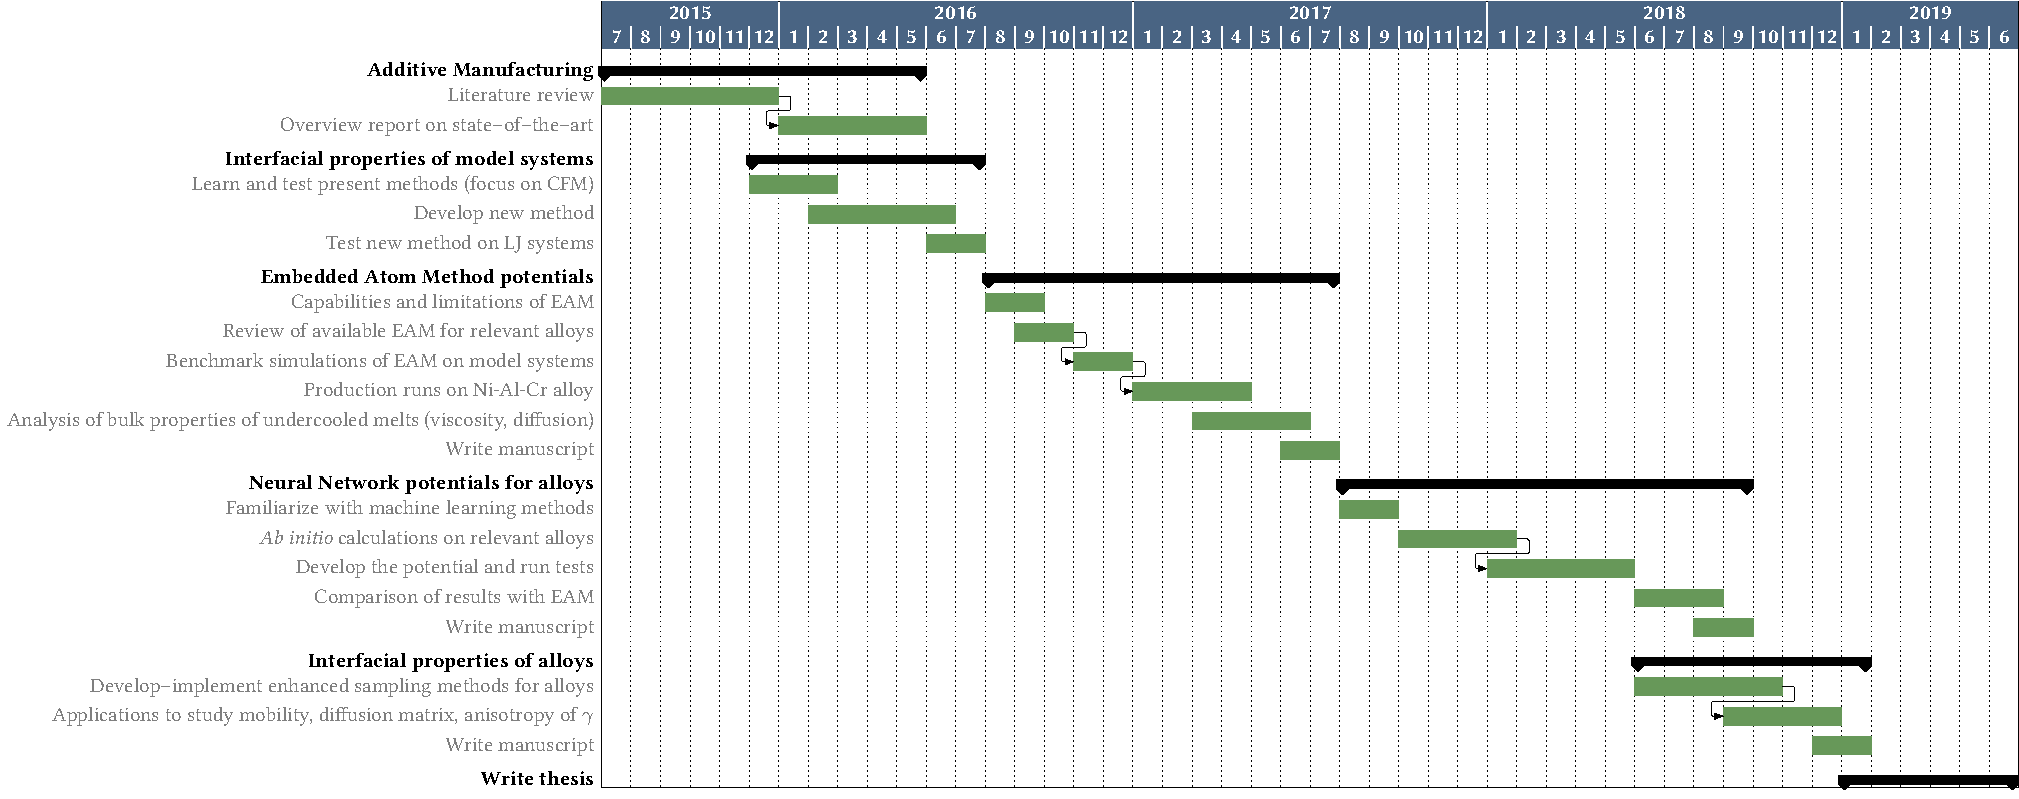
\includegraphics[angle=90,height=0.79\textheight]{Gantt-standalone.pdf}
%    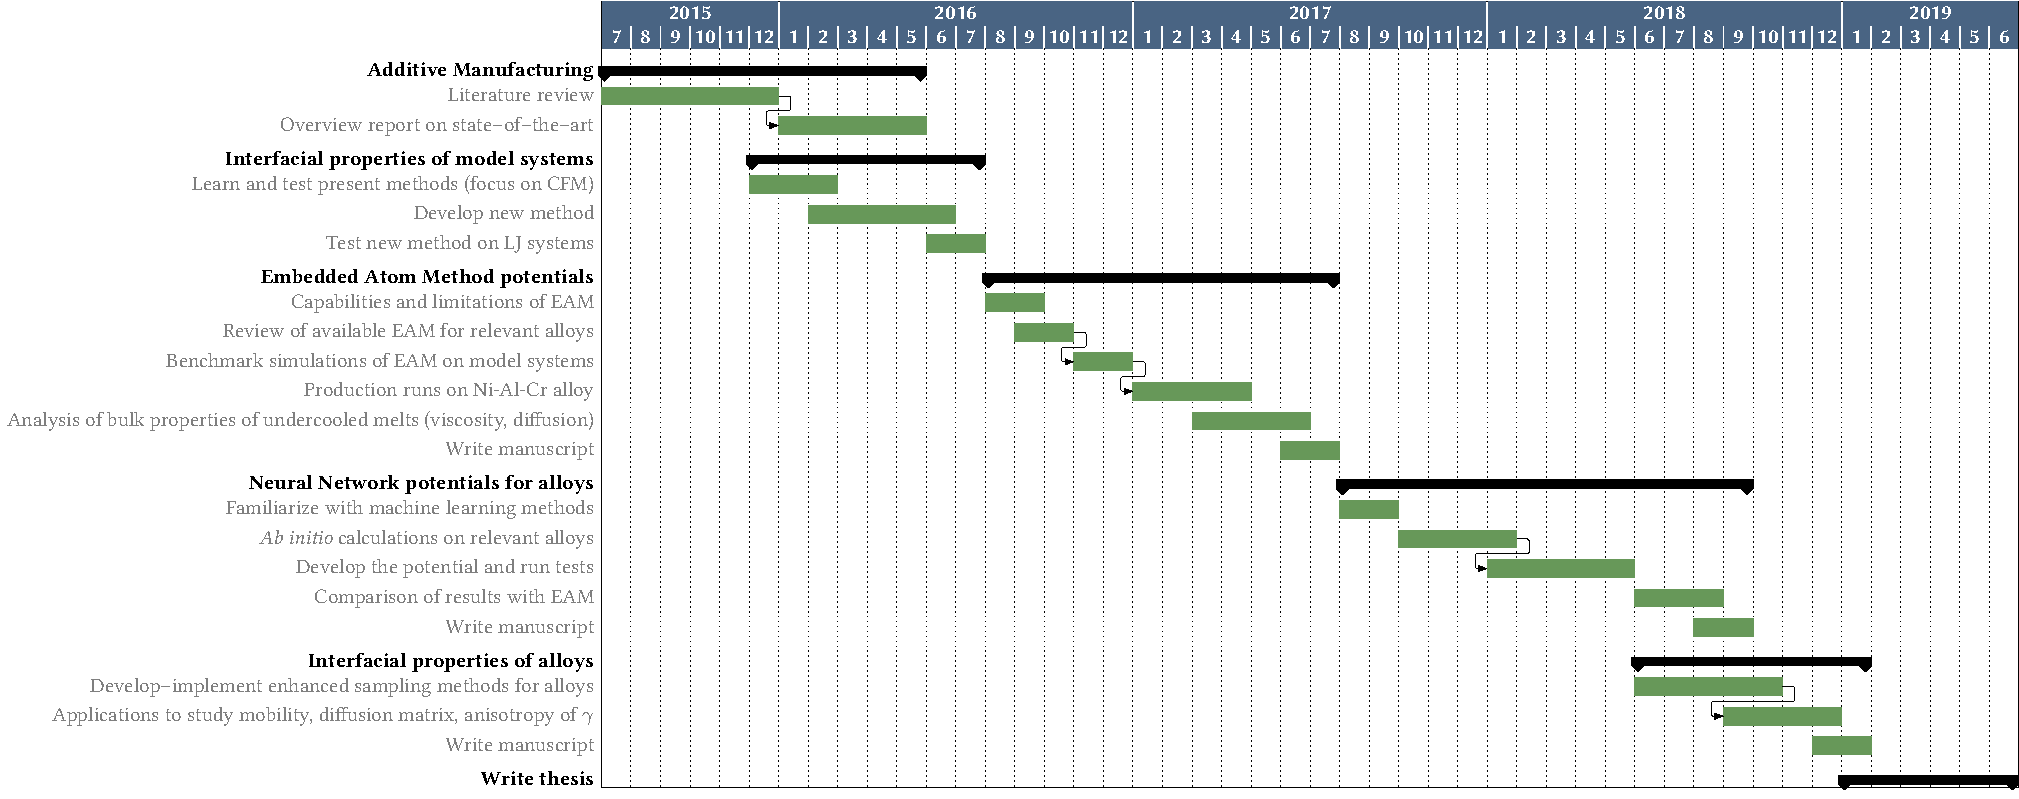
\includegraphics[width=\textwidth]{Gantt-standalone.pdf}
%\end{center}
\begin{figure}[h]
    \centering
    \resizebox{\Textht}{!}{%
        \begin{tikzpicture}
\begin{ganttchart}[
        y unit title=0.4cm,
        y unit chart=0.5cm,
        vgrid,
        time slot format=simple,
        %compress calendar,
        title/.append style={draw=none, fill=RoyalBlue!50!black},
        title label font=\sffamily\bfseries\color{white},
        title label node/.append style={below=-1.6ex},
        title left shift=.05,
        title right shift=-.05,
        title height=1,
        bar/.append style={draw=none, fill=OliveGreen!75},
        bar height=.6,
        bar label font=\normalsize\color{black!70},
        group right shift=0,
        group top shift=.6,
        group height=.3,
        group peaks height=.2,
        bar incomplete/.append style={fill=Maroon}
        ]{1}{48}
    \gantttitle{2015}{6}
    \gantttitle{2016}{12}
    \gantttitle{2017}{12}
    \gantttitle{2018}{12}
    \gantttitle{2019}{6} \\
    %
    \gantttitlelist{7,...,12}{1}
    \gantttitlelist{1,...,12}{1}
    \gantttitlelist{1,...,12}{1}
    \gantttitlelist{1,...,12}{1}
    \gantttitlelist{1,...,6}{1} \\
    %
    \ganttgroup{Additive Manufacturing}{1}{11} \\
    \ganttbar{Literature review}{1}{6} \\
    \ganttlinkedbar{Overview report on state--of--the--art}{7}{11}
    \ganttnewline
    %
    \ganttgroup{Interfacial properties of model systems}{6}{13}\\
    \ganttbar{Learn and test present methods (focus on CFM)}{6}{8}\\
    \ganttbar{Develop new method}{8}{12}\\
    \ganttbar{Test new method on LJ systems}{12}{13}
    \ganttnewline
    %
    \ganttgroup{Embedded Atom Method potentials}{14}{25}\\
    \ganttbar{Capabilities and limitations of EAM}{14}{15}\\
    \ganttbar{Review of available EAM for relevant alloys}{15}{16}\\
    \ganttlinkedbar{Benchmark simulations of EAM on model systems}{17}{18}\\
    \ganttlinkedbar{Production runs on Ni-Al-Cr alloy}{19}{22}\\
    \ganttbar{Analysis of bulk properties of undercooled melts (viscosity, diffusion)}{21}{24}\\
    \ganttbar{Write manuscript}{24}{25}
    \ganttnewline
    %
    \ganttgroup{Neural Network potentials for alloys}{26}{39}\\
    \ganttbar{Familiarize with machine learning methods}{26}{27}\\
    \ganttbar{\textit{Ab initio} calculations on relevant alloys}{28}{31}\\
    \ganttlinkedbar{Develop the potential and run tests}{31}{35}\\
    \ganttbar{Comparison of results with EAM}{36}{38}\\
    \ganttbar{Write manuscript}{38}{39}\ganttnewline
    %
    \ganttgroup{Interfacial properties of alloys}{36}{43}\\
    \ganttbar{Develop--implement enhanced sampling methods for alloys}{36}{40}\\
    \ganttlinkedbar{Applications to study mobility, diffusion matrix, anisotropy of $\gamma$}{39}{42}\\
    \ganttbar{Write manuscript}{42}{43}\ganttnewline
    %
    \ganttgroup{Write thesis}{43}{48}
    %%%%
    %\ganttmilestone{Milestone}{7} \ganttnewline
    %\ganttbar{Final Task}{8}{12}
    %\ganttlink{elem2}{elem3}
    %\ganttlink{elem3}{elem4}
\end{ganttchart}
\end{tikzpicture}
    }
\end{figure}
\end{landscape}